\chapter{Overview}\label{ch:overview}

\section{Introduction}\label{sec:1-introduction}

In modern embedded systems (Embedded System), as the demands on computation grow, the prevalence of multi-core systems is increasing rapidly, and at the same time the trend of heterogeneous computing is becoming ever more pronounced. At the same time, the functional complexity and market share of microcontroller systems with markedly different architectures are rising rapidly, and the requirements for resource management are also growing. However, for multi-core systems, while computing capability grows, their real-time responsiveness is often impaired by resource access contention, so it is necessary to write a fully parallel kernel that is lock-free and has little shared state; for microcontroller (Microcontroller Unit, MCU) systems, their memory management approaches differ, and the traditional abstraction methods often cannot meet the requirements, so it is impossible to use the same system-level programming paradigm as medium and large computers, and it is therefore necessary to write a new system to unify the memory management interface.

At the same time, in modern high-performance systems, the importance of lightweight virtualization functionality is gradually increasing. In large servers, virtualization can make resource management more flexible, and can further enable applications such as hot migration of virtual machines, facilitating hardware maintenance; in high-performance embedded systems, virtualization (Virtualization) can allow microcontrollers or digital signal processors (Digital Signal Processor, DSP) to securely run third-party binary code, or to run multiple high-level language virtual machines, without causing security and resource control problems. In both scenarios, virtual machines are required to respond in real time, to be highly efficient, and to be scalable and extensible.

RME (RTOS-Mutate-Eukaron) real-time operating system (Real-Time Operating System, RTOS) is an extremely scalable (Scalable) and expandable (Expandable) fully preemptive microkernel real-time operating system. It provides all the features provided by third-generation microkernels: a flexible user-mode scheduler, complete low-level storage management, efficient communication mechanisms, and special optimization capabilities for specific hardware. The RME operating system can run on microcontrollers with only 64kB of read-only memory (Read-Only Memory, ROM) and 16kB of random-access memory (Random-Access Memory, RAM), and can also run on high-performance servers with hundreds of CPU sockets and hundreds of TB of memory, while possessing equally superior operating efficiency.

\subsection{Design Goals}\label{subsec:1-design-goals}

As a third-generation microkernel, the design goals of RME mainly include the following four points: flexibility, security, reliability and real-time responsiveness.

Flexibility (Flexibility) means that the system can adapt to a variety of application scenarios, and fully exploit the potential of various architectures when running on them, while using as many common parts as possible. To this end, RME was designed with a range of possible platforms, from microcontrollers to supercomputers, in mind, and follows strict coding compatibility specifications to accommodate all possible compilation environments.

Security (Security) means the controlled confidentiality (Confidentiality), integrity (Integrity) and availability (Availability) of the various resources in the system. To achieve the above three requirements, RME takes capabilities (Capability) as the foundation of the system. This means that, in the system, everything is controlled and managed by capabilities; to operate on a kernel object, the corresponding capability must be passed in through a system call. At user level, different kernel object managers manage different categories of capabilities, so their coupling is very low, and consequently the degree of isolation between them is relatively high.

Reliability (Reliability) means that there are few or no functional errors in the system, and that when such errors occur, a micro-reboot (Micro-reboot) of the subsystem can be performed. As a microkernel, RME is inherently more reliable than monolithic kernels; to minimize the occurrence of errors, the architecture-independent part of the RME code has all been subjected to white-box testing with full branch coverage.

Real-time responsiveness (Real-time Responsiveness) means that all execution paths in the system are bounded by definite time limits, and these limits are short enough not to cause problems. RME was designed with the predictability of all execution paths in mind, and can maintain its own hard real-time responsiveness even in multi-core environments.

\subsection{Software Copyright and License}\label{subsec:1-copyright-and-license}

Taking comprehensive account of the different requirements of microcontroller applications, deeply embedded applications and traditional applications on open-source systems, the license adopted by the RME kernel itself is Unlicensed, but special provisions apply to some special cases\footnote{Such as security equipment and medical equipment, etc.} These special provisions are case-specific, and the specific terms will differ for each possible situation.

\subsection{Glossary of Easily Confused Terms}\label{subsec:1-terms-and-definitions}

In this book, the basic terms that are easily confused are defined as follows:

\subsubsection{Operating System}\label{subsubsec:1-operating-system}

Refers to the basic software running on a device that performs the lowest-level management of hardware resources such as the processor and memory.

\subsubsection{Process}\label{subsubsec:1-process}

A process refers to the smallest independent protection space that possesses certain resources. These resources can be certain kernel objects, a certain range of memory, certain devices, etc. Generally speaking, this protection space will correspond to an instance of a program that is currently executing.

\subsubsection{Thread}\label{subsubsec:1-thread}

A thread refers to a schedulable entity in an operating system that possesses an independent execution stack and an independent instruction stream. A process can contain multiple threads, and they share one process address space.

\subsubsection{Coroutine}\label{subsubsec:1-coroutine}

A coroutine refers to a schedulable entity in an operating system that possesses only an independent instruction stream but no independent stack. A thread can contain multiple coroutines, and these coroutines share one thread stack.

\subsubsection{Static Allocation}\label{subsubsec:1-static-allocation}

Refers to an allocation method in which the resource allocation scheme is decided at system compile time.

\subsubsection{Semi-Static Allocation}\label{subsubsec:1-semi-static-allocation}

Refers to an allocation method in which the resource allocation scheme is decided during system startup and is not changed afterwards during runtime.

\subsubsection{Dynamic Allocation}\label{subsubsec:1-dynamic-allocation}

Refers to an allocation method in which the resource allocation can be changed during system runtime.

\subsubsection{Soft Real-Time}\label{subsubsec:1-soft-real-time}

Refers to a real-time guarantee in which operations should be completed within their deadlines in the vast majority of cases, but a small portion of operations is also allowed to occasionally complete beyond their deadlines.

\subsubsection{Hard Real-Time}\label{subsubsec:1-hard-real-time}

Refers to a real-time guarantee in which all operations must be completed within their deadlines.

\subsubsection{Constant Real-Time}\label{subsubsec:1-constant-real-time}

Refers to a real-time guarantee in which all operations are O(1) with respect to user input and system configuration, and all executions can be completed within some practically meaningful constant time limit. This is the strongest of all real-time guarantees.

\subsubsection{Constant Real-Time to a Certain Value}\label{subsubsec:1-value-constant-real-time}

Refers to a real-time guarantee in which all operations and responses are O(1) while a certain value that can be determined by the system configuration remains unchanged, and all executions can be completed within some practically meaningful constant time limit.

\subsection{Major Reference Systems}\label{subsec:1-major-reference-systems}

The capability table, signal endpoint and synchronous invocation take Composite (@GWU) as a reference.

Part of the implementation of the page table takes Composite (@GWU) as a reference.

The dynamic page functionality of the page table takes uCLinux (@Emcraft) as a reference.

The concept of kernel memory capabilities takes Fiasco.OC (@TU Dresden) as a reference.

The operation flags of capabilities and the implementation of the maximum priority of threads take seL4 (@Data61/CSIRO) as a reference.

The implementation of the lightweight scheduling queues in the kernel takes RMProkaron (@EDI) as a reference.

The implementation of the system call interface takes Linux (@The Linux Foundation/Linus Torvalds) as a reference.

The implementation of the separation kernel takes Barrelfish (@Microsoft/ETH Zurich) as a reference.

The references and reference materials for the other chapters are listed in those chapters.

\section{Foreword}\label{sec:1-foreword}

An operating system is a kind of basic software running on a device that performs the lowest-level management of hardware resources such as the processor and memory. For a real-time operating system, every operation of the system must be correct and timely, and its execution time must be predictable. Generally speaking, there are two types of real-time operating systems: the first is soft real-time systems, and the second is hard real-time systems. For a soft real-time system, it suffices that the responses of the program are within their deadlines in most cases; for a hard real-time system, the responses of the system must be within their deadlines at all times. In reality, few real-time applications or operating systems are entirely soft real-time or entirely hard real-time; they are usually an organic combination of a soft real-time part and a hard real-time part. For example, the LCD display and human-machine interface part is usually soft real-time, while the motor control part is usually hard real-time.

Generally speaking, the vast majority of real-time systems are embedded systems. An embedded system refers to a dedicated system that is highly customized in both software and hardware, and it imposes very stringent requirements on the system's performance, power consumption, size and operating environment. Such systems include highly customized systems such as industrial automation controllers, flight controllers and rocket controllers, as well as relatively general-purpose systems such as industrial control computers.

Traditionally, owing to the limitations of hardware capabilities, real-time systems were generally rather simple, and it was feasible to cope with them using a simple operating system or no operating system at all. At present, with the introduction of new-generation microcontrollers and microprocessors, the complexity of application software has greatly increased, which makes the use of new-generation real-time operating systems inevitable.

The new generation of real-time operating systems is more powerful than existing real-time systems in aspects such as reliability, portability and flexibility, especially with regard to the utilization of multi-core processors and to the design of and consideration for parallelization. Taking these design requirements into account, a microkernel is an inevitable choice. A microkernel implements a minimal set of primitives, which can be used to place the vast majority of the functionality that traditional operating systems keep in kernel mode into user-mode servers. If one of the drivers or servers fails, we can often confine the fault to a small scope so that it does not spread to the entire operating system. Therefore, the various user-mode servers can be restarted individually and can also be redundantly backed up, greatly improving the security and reliability of the system.

Moreover, a microkernel generally makes the writing of multi-core parallel-related code easier, because the kernel is simple and the number of synchronization mechanisms that need to be added is smaller. This enables us to make extensive use of read-modify-write (Read-Copy-Update, RCU) techniques, making it possible to write a lock-free kernel. Furthermore, because the capabilities of the microkernel are all placed in tables and aligned to a cache line, we can always avoid the false-sharing (False-sharing) problem caused by cache coherence, thereby greatly improving the kernel's performance under multi-processor or multi-node non-uniform memory access architectures (Non-Uniform Memory Access, NUMA).

Here we review the categories of operating systems. In this manual, we divide common operating systems into five categories, respectively called fully customized systems, ultra-lightweight systems, basic real-time systems, complex application systems and complex real-time application systems. Below we will introduce the concepts of these operating systems respectively.

\subsection{Fully Customized Systems}\label{subsec:1-fully-customized-systems}

Such systems are operating systems fully customized for a certain application. They do not possess system services and software abstraction layers in the sense of general operating systems, nor do they possess a distinction between kernel space and user space; applications run directly on the bare metal. Generally speaking, unikernels (Unikernel) all belong to this category. The vast majority of microcontroller foreground/background bare-metal processing systems also belong to this category.

Typical such operating systems include Rump (unikernel) and Mirage OS (unikernel).

\subsection{Ultra-Lightweight Systems}\label{subsec:1-ultra-lightweight-systems}

An ultra-lightweight system is the minimal system that can be called an operating system. Generally speaking, it usually runs on 8-bit or even 4-bit machines, does not require a system timer, has no distinction between kernel mode and user mode, and can run on multiple architectures without porting. It usually consists of only a small piece of code responsible for task switching or even just a few macros, and can be compiled and run without a customized linker script.

It generally consists of a while() main loop, and in that loop it calls the task functions one by one. The task functions are simple state machines, and each time one is entered it selects a state to run. The various tasks use the same stack. The task code is compiled together with the kernel. The tasks behave as cooperative coroutines that cannot preempt one another, and they do not need to be reentrant.

Its priority system is implemented using the priority configuration of hardware interrupts, and the hardware interrupt functions directly process everything rather than deferring processing to tasks. Interrupts are completely transparent to the operating system, and the operating system does not need to know whether an interrupt has arrived.

Typical such operating systems include EDI's RMS (ultra-lightweight coroutine library) and FAU's Sloth (enhanced lightweight coroutine library).

\subsection{Basic Real-Time Systems}\label{subsec:1-basic-real-time-systems}

A basic real-time system is the minimal system that preliminarily exhibits the basic characteristics of real-time systems. It generally runs on high-end 8/16-bit machines and low-end 32-bit machines, and requires a system timer. It has no distinction between user mode and kernel mode, but the memory management unit (Memory Management Unit, MMU) or memory protection unit (Memory Protection Unit, MPU) can be configured to protect a certain range of memory. It requires simple architecture-dependent assembly code to perform context stack switching. To make it runnable on multiple architectures, modifying this piece of assembly code is mandatory. Porting also often involves the system timer, stack switching, interrupt management and coprocessor management. Such systems may or may not use a customized linker script; generally speaking, a customized linker script must be used when memory protection is involved.

In such systems, tasks present themselves as threads. Task functions may be reentrant. Each task uses a separate execution stack. The task code and the kernel code may or may not be compiled together. Tasks calling system functions usually use direct ordinary function calls; there is no concept of making system calls via software interrupts.

Such systems possess the concept of priority, and generally implement preemption between different priorities and timeslice round-robin scheduling among the same priority. Such systems possess a rudimentary memory management scheme, and this memory management scheme is generally based on SLAB and the buddy system.

Interrupts may be completely transparent to the operating system, in which case the operating system does not need to know whether an interrupt has arrived; if a context switch needs to be performed in an interrupt, the stack switching assembly must be inserted into that interrupt function, in which case the interrupt entry and exit need to be written in assembly code.

Typical such operating systems include RMP, RT-Thread, FreeRTOS, uC/OS, Salvo and ChibiOS.

\subsection{Complex Application Systems}\label{subsec:1-complex-application-systems}

A complex application system is a system that exhibits most of the characteristics of an operating system, but its real-time metrics are generally not outstanding. It generally runs on 32-bit and 64-bit machines, and requires a system timer. It has a strict distinction between kernel mode and user mode, and requires that the hardware it runs on must have an MMU or MPU. It requires a fairly complex customized linker script, and requires extensive porting before it can run on a new architecture. Porting mainly involves the system timer, context/protection domain switching, interrupt management and coprocessor management, etc.

On such systems, tasks present themselves as processes, and one task can contain multiple threads. Because virtual memory is used, whether the task functions are reentrant has no impact. The kernel code and the applications are compiled separately. System calls are made through software interrupts or dedicated system call instructions\footnote{Such as SYSCALL, SYSRET, etc. on x86-64}.

Such systems possess the concept of priority, but real-time performance is generally not guaranteed.

Such systems generally have two-level memory management. At the lower level is the management of pages, and at the upper level is the stack management provided by the system runtime library.

Interrupts are not transparent to such systems. The operating system requires that the context registers, coprocessors and MMU/MPU be maintained when entering and exiting an interrupt.

Typical such operating systems include Windows, Linux, Minix, FreeBSD, MacOS X and Amiga.

\subsection{Complex Real-Time Application Systems}\label{subsec:1-complex-real-time-application-systems}

Complex real-time application systems are the most powerful category of all operating systems. The main characteristic of such systems is that, on top of complex application systems, guarantees of real-time responsiveness are added, and the execution timing of the kernel is completely predictable.

Typical such operating systems include RME, Composite, Fiasco.OC and various other L4 systems, RTLinux and VxWorks. RME is designed as such a system. Therefore, its design needs to take the most issues into account, and its design difficulty is also the greatest.

In the designs of the kernels described in \ref{subsec:1-basic-real-time-systems} and \ref{subsec:1-complex-application-systems}, there have always been two approaches, namely the monolithic kernel (Monolithic Kernel) and the microkernel (Microkernel). The representative of the former is Linux, which compiles and links all system services into kernel space. The advantage of doing so is that all inter-module calls are simple function calls with no cross-protection-domain overhead, so it is faster; moreover, the kernel itself can provide more functionality. The representative of the latter is the various L4s, which place all functionality in user space as much as possible, and the kernel itself is only responsible for basic functions such as message forwarding and scheduling. In later microkernel development, even the scheduler and kernel memory management were further placed in user space. The advantage of doing so is that the functional modules of the operating system are isolated from one another as much as possible, achieving better maintainability, security and reliability, and the attack surface exposed to hackers is also smaller; the kernel itself can moreover undergo formal verification (Formal Verification) to guarantee its correctness\hyperref[cite:1-4]{{[}4{]}}. The typical system architecture diagrams of these two approaches are shown below:

\begin{figure}[htbp]
    \centering
    \includegraphics[width=0.72\textwidth]{Figure/image2.pdf}
    \caption{Monolithic Kernel Architecture}
    \label{fig:1-1-monolithic-kernel-architecture}
\end{figure}

\begin{figure}[htbp]
    \centering
    \includegraphics[width=0.72\textwidth]{Figure/image3.pdf}
    \caption{Microkernel Architecture}
    \label{fig:1-2-microkernel-architecture}
\end{figure}

RME adopts a microkernel design. On the one hand, the advantage of monolithic kernels in not needing to frequently cross protection domains has become very insignificant on modern architectures\footnote{For example, the dedicated system call instruction pair SYSCALL and SYSRET of the latest x86-64 consumes only 60 cycles, equivalent to one L3 cache miss}, while on the other hand, microkernels, owing to the excellent locality of code and data and their simple internal structure, have achieved a decisive advantage in cache performance and concurrency performance, causing monolithic kernels to lose their only advantage------speed. A group of microkernel operating systems recently developed, represented by seL4\hyperref[cite:1-4]{{[}4{]}}, can be dozens of times better than Linux in inter-process communication, and their worst-case response time, depending on the configuration, can be even better. In terms of application performance, network function virtualization (Network Function Virtualization, NFV) applications based on microkernels have also achieved performance generally an order of magnitude higher than Linux, thoroughly refuting the assertion that monolithic kernels necessarily have high performance.

As for RME itself, on some single-core architectures\footnote{Especially a group of microcontrollers represented by Cortex-M} its average inter-process communication performance is 40 times that of Linux; even including the overhead caused by the user-mode library, it is still 25 times faster than Linux.

\section{Performance Metrics of Real-Time Operating Systems and Their Components}\label{sec:1-rtos-performance-metrics}

There are hundreds of different kinds of RTOSes on the current market, and kernels developed by hobbyists and individuals are even more numerous. The performance of these systems often varies greatly. We need some metrics to measure the performance of these RTOSes. The metrics listed below can only be compared directly when the processor architecture, compiler and compilation options are the same. If different architectures, compilers or compilation options are used, the resulting data have no direct meaning, and are only for reference and not comparable. One recommended method is to evaluate using industry-standard ARM or MIPS series processors together with the GCC-O2 option. In addition, the Chronos simulator together with GCC-O2 can also be used for evaluation. When evaluating, note also that the load level of the system may affect these values, so these values can be compared only when the load level of the system is the same.

\subsection{Kernel Size}\label{subsec:1-kernel-size}

Kernel size is an important metric for measuring RTOSes. Because RTOSes are usually deployed on devices with extremely limited memory, a small kernel size is critical. Kernel size is mainly measured from two aspects, the first being the read-only segment size and the second being the data segment size. The read-only segment includes the kernel's code segment and read-only data segment, and the data segment includes the size of the kernel's read-write data segment. In Flash-based microcontroller systems, the read-only segments consume Flash, while the data segments consume SRAM.\hyperref[cite:1-1]{{[}1{]}}

Because RTOSes are highly configurable, their kernel size is often not fixed, but is closely related to the configuration chosen. Therefore, to measure this performance, one should examine the kernel size under the minimal kernel configuration, the common kernel configuration and the maximal kernel configuration.\hyperref[cite:1-1]{{[}1{]}}

Obtaining kernel size data is very simple: just compile the kernel with a compiler, and then use a dedicated binary viewer\footnote{Such as Objdump} to inspect the size of each section of the target file.

\subsection{Execution Time, Worst-Case Execution Time and Their Jitter}\label{subsec:1-execution-time-and-jitter}

Execution time refers to the amount of time an RTOS system call takes. Worst-case execution time refers to the maximum length that the execution time can reach under the most unfavorable conditions. The worst-case execution time of an RTOS is usually reached under the following circumstances: the most time-consuming system call is executed, and a large number of cache misses and TLB misses occur in the process. RTOSes generally disable interrupts when executing system calls; the worst-case execution time is usually the longest time the system keeps interrupts disabled, so its impact on the system's real-time responsiveness is enormous.

Worst-case execution time can be divided into two categories: the first is the worst-case execution time of kernel system calls, and the other is the worst-case execution time of inter-process communication and inter-thread synchronization.

To obtain the first type of worst-case execution time, before calling a certain system call, the timer can record the timestamp T\textsubscript{s} at this time, and then after the system call ends, the timer is called again to record the timestamp T\textsubscript{e} at this time. Then, the timer is called twice in succession, recording two timestamps T\textsubscript{ts} and T\textsubscript{te}, yielding the extra cost of calling the timer as T\textsubscript{te}-T\textsubscript{ts}. At this point, the execution time is T\textsubscript{e}-T\textsubscript{s}-(T\textsubscript{te}-T\textsubscript{ts}). The worst-case execution time is the largest execution time among all the system call tests.

To obtain the second type of worst-case execution time, the timer can be called once at the sending end of the communication mechanism to record the timestamp T\textsubscript{s} at this time, and called once at the receiving end of the communication mechanism to record the timestamp T\textsubscript{e} at this time. The measurement of the cost of calling the timer is similar to that for the first type of worst-case execution time. The finally obtained T\textsubscript{e}-T\textsubscript{s}-(T\textsubscript{te}-T\textsubscript{ts}) is the execution time. The worst-case execution time is the largest execution time among all the communication tests.

The jitter of execution time is also very important. When measuring the execution and communication time of the same system multiple times, we often obtain a distribution. The mean of this distribution is the average execution time, and its standard deviation\footnote{Sometimes we also use the range} is called the execution time jitter.

For an RTOS, we generally consider that the execution time, the worst-case execution time and the jitter are all better the smaller they are. Execution time can be further divided in detail into the following categories:\hyperref[cite:1-1]{{[}1{]}}

\subsubsection{Intra-Process Thread Switch Time}\label{subsubsec:1-intra-process-thread-switch}

Intra-process thread switch time refers to the time consumed to switch from one thread to another within the same process. We measure it using the method shown below. In the measurement, in addition to the method using T\textsubscript{e}-T\textsubscript{s}, the difference between two consecutive T\textsubscript{s} values divided by 2 can also be used. Thread switching includes two cases: one is switching between threads of the same priority, and the other is waking up a higher-priority thread from a lower-priority thread.\hyperref[cite:1-2]{{[}2{]}}

In the first case, we assume that the two threads in the figure have the same priority, and that at the start of the measurement we are executing thread A, which has just been switched to by thread B.

\begin{xltabular}{\textwidth}{@{}>{\hsize=1.0000\hsize\raggedright\arraybackslash}X>{\hsize=1.0000\hsize\raggedright\arraybackslash}X@{}}
\caption{The First Case of Intra-Process Thread Switching}\label{tab:1-1-intra-process-thread-switch-case-1}\\
\toprule
Process 1: Thread A & Process 1: Thread B\tabularnewline
\endfirsthead
\toprule
Process 1: Thread A & Process 1: Thread B\tabularnewline
\midrule
\endhead
\bottomrule
\endlastfoot
Loop forever

\{

\textgreater\textgreater{} Record time T\textsubscript{s};

Switch to thread B;

\}\strut
 & Loop forever

\{

Record time T\textsubscript{e};

\textgreater\textgreater{} Switch to thread A;

\}\strut
\tabularnewline
\end{xltabular}
\nopagebreak[4]

In the second case, we assume that thread B in the figure has a higher priority, and that at the start of the measurement we are executing thread A, which has just been switched to by thread B.

\begin{xltabular}{\textwidth}{@{}>{\hsize=1.0045\hsize\raggedright\arraybackslash}X>{\hsize=0.9955\hsize\raggedright\arraybackslash}X@{}}
\caption{The Second Case of Intra-Process Thread Switching}\label{tab:1-2-intra-process-thread-switch-case-2}\\
\toprule
Process 1: Thread A & Process 1: Thread B\tabularnewline
\endfirsthead
\toprule
Process 1: Thread A & Process 1: Thread B\tabularnewline
\midrule
\endhead
\bottomrule
\endlastfoot
Loop forever

\{

\textgreater\textgreater{} Record time T\textsubscript{s};

Wake up B (conventional) or switch to B (microkernel);

\}\strut
 & Loop forever

\{

Record time T\textsubscript{e};

\textgreater\textgreater{} Sleep (conventional) or switch to A (microkernel);

\}\strut
\tabularnewline
\end{xltabular}
\nopagebreak[4]

\subsubsection{Inter-Process Thread Switch Time}\label{subsubsec:1-inter-process-thread-switch}

Inter-process thread switch time refers to the time consumed to switch from one thread to another between different processes. The measurement method and the two possible cases are completely identical to those described in the previous section; the only difference is that the threads participating in the test now belong to two processes.\hyperref[cite:1-2]{{[}2{]}}

In the first case, we assume that the two threads in the figure have the same priority, and that at the start of the measurement we are executing

thread A, which has just been switched to by thread B.

\begin{xltabular}{\textwidth}{@{}>{\hsize=1.0000\hsize\raggedright\arraybackslash}X>{\hsize=1.0000\hsize\raggedright\arraybackslash}X@{}}
\caption{The First Case of Inter-Process Thread Switching}\label{tab:1-3-inter-process-thread-switch-case-1}\\
\toprule
Process 1: Thread A & Process 2: Thread B\tabularnewline
\endfirsthead
\toprule
Process 1: Thread A & Process 2: Thread B\tabularnewline
\midrule
\endhead
\bottomrule
\endlastfoot
Loop forever

\{

\textgreater\textgreater{} Record time T\textsubscript{s};

Switch to thread B;

\}\strut
 & Loop forever

\{

Record time T\textsubscript{e};

\textgreater\textgreater{} Switch to thread A;

\}\strut
\tabularnewline
\end{xltabular}
\nopagebreak[4]

In the second case, we assume that thread B in the figure has a higher priority, and that at the start of the measurement we are executing thread A, which has just been switched to by thread B.

\begin{xltabular}{\textwidth}{@{}>{\hsize=1.0044\hsize\raggedright\arraybackslash}X>{\hsize=0.9956\hsize\raggedright\arraybackslash}X@{}}
\caption{The Second Case of Inter-Process Thread Switching}\label{tab:1-4-inter-process-thread-switch-case-2}\\
\toprule
Process 1: Thread A & Process 2: Thread B\tabularnewline
\endfirsthead
\toprule
Process 1: Thread A & Process 2: Thread B\tabularnewline
\midrule
\endhead
\bottomrule
\endlastfoot
Loop forever

\{

\textgreater\textgreater{} Record time T\textsubscript{s};

Wake up B (conventional) or switch to B (microkernel);

\}\strut
 & Loop forever

\{

Record time T\textsubscript{e};

\textgreater\textgreater{} Sleep (conventional) or switch to A (microkernel);

\}\strut
\tabularnewline
\end{xltabular}
\nopagebreak[4]

\subsubsection{Intra-Process Inter-Thread Synchronous Communication Time}\label{subsubsec:1-intra-process-sync-communication}

Intra-process inter-thread synchronous communication time refers to the total time used to perform synchronous communication between different threads within the same process. The following measurement assumes that thread B has already blocked at the receiving end, thread A performs the send, and thread B has a higher priority than thread A. For systems that communicate using thread migration techniques\footnote{Such as RME and some L4 series}, the measurement of this parameter is meaningless, because synchronous communication is not needed within a process.\hyperref[cite:1-2]{{[}2{]}}

\begin{xltabular}{\textwidth}{@{}>{\hsize=1.0000\hsize\raggedright\arraybackslash}X>{\hsize=1.0000\hsize\raggedright\arraybackslash}X@{}}
\caption{Intra-Process Inter-Thread Synchronous Communication}\label{tab:1-5-intra-process-sync-communication}\\
\toprule
Process 1: Thread A & Process 1: Thread B\tabularnewline
\endfirsthead
\toprule
Process 1: Thread A & Process 1: Thread B\tabularnewline
\midrule
\endhead
\bottomrule
\endlastfoot
Loop forever

\{

\textgreater\textgreater{} Record time T\textsubscript{s};

Send a signal to synchronous endpoint P;

\}\strut
 & Loop forever

\{

Record time T\textsubscript{e};

\textgreater\textgreater{} Receive a signal from synchronous endpoint P;

\}\strut
\tabularnewline
\end{xltabular}
\nopagebreak[4]

\subsubsection{Inter-Process Synchronous Communication Time}\label{subsubsec:1-inter-process-sync-communication}

Inter-process synchronous communication time refers to the total time used to perform synchronous communication between different processes. The following measurement applies to traditional operating systems, and assumes that thread B has already blocked at the receiving end, thread A performs the send, and thread B has a higher priority than thread A.\hyperref[cite:1-2]{{[}2{]}}

\begin{xltabular}{\textwidth}{@{}>{\hsize=1.0000\hsize\raggedright\arraybackslash}X>{\hsize=1.0000\hsize\raggedright\arraybackslash}X@{}}
\caption{Inter-Process Synchronous Communication of Traditional Operating Systems}\label{tab:1-6-inter-process-sync-communication}\\
\toprule
Process 1: Thread A & Process 2: Thread B\tabularnewline
\endfirsthead
\toprule
Process 1: Thread A & Process 2: Thread B\tabularnewline
\midrule
\endhead
\bottomrule
\endlastfoot
Loop forever

\{

\textgreater\textgreater{} Record time T\textsubscript{s};

Send a signal to synchronous endpoint P;

\}\strut
 & Loop forever

\{

Record time T\textsubscript{e};

\textgreater\textgreater{} Receive a signal from synchronous endpoint P;

\}\strut
\tabularnewline
\end{xltabular}
\nopagebreak[4]

For operating systems such as RME and L4 that employ thread migration techniques, the measurement is as follows. Note that when thread A migrates and invokes function F, we are still running inside thread A, except that the code segment being executed and the data segment being used have moved into another process, and an additionally allocated execution stack is used inside that process.

\begin{xltabular}{\textwidth}{@{}>{\hsize=1.0994\hsize\raggedright\arraybackslash}X>{\hsize=0.9006\hsize\raggedright\arraybackslash}X@{}}
\caption{Inter-Process Synchronous Communication with Thread Migration Techniques}\label{tab:1-7-thread-migration-sync-communication}\\
\toprule
Process 1: Thread A & Process 2: Thread A\tabularnewline
\endfirsthead
\toprule
Process 1: Thread A & Process 2: Thread A\tabularnewline
\midrule
\endhead
\bottomrule
\endlastfoot
Loop forever

\{

\textgreater\textgreater{} Record time T\textsubscript{s};

Migrate and invoke function F;

\}\strut
 & Function F

\{

Record time T\textsubscript{e};

Return;

\}\strut
\tabularnewline
\end{xltabular}
\nopagebreak[4]

\subsubsection{Intra-Thread Asynchronous Communication Time}\label{subsubsec:1-intra-thread-async-communication}

Intra-thread asynchronous communication time refers to the total time used to send and receive asynchronous signals within the same thread. Common asynchronous signals may include the asynchronous signal primitive (Signal) provided by the RME system, or the semaphore (Semaphore), mailbox (Mailbox), message queue (Queue), pipe (Pipe), etc. provided by other operating systems. We measure it using the method shown below.\hyperref[cite:1-2]{{[}2{]}}
In the final measurement results, T\textsubscript{i}-T\textsubscript{s} yields the time consumed by the send, T\textsubscript{e}-T\textsubscript{i} yields the time consumed by the receive, and T\textsubscript{e}-T\textsubscript{i} is the communication time.

\begin{xltabular}{\textwidth}{@{}>{\hsize=1.0000\hsize\raggedright\arraybackslash}X@{}}
\caption{Intra-Thread Asynchronous Communication}\label{tab:1-8-intra-thread-async-communication}\\
\toprule
Thread A\tabularnewline
\endfirsthead
\toprule
Thread A\tabularnewline
\midrule
\endhead
\bottomrule
\endlastfoot
Loop forever

\{

Record time T\textsubscript{s};

Send a signal to asynchronous endpoint P;

Record time T\textsubscript{i};

Receive a signal from asynchronous endpoint P;

Record time T\textsubscript{e};

\}\strut
\tabularnewline
\end{xltabular}
\nopagebreak[4]

\subsubsection{Intra-Process Inter-Thread Asynchronous Communication Time}\label{subsubsec:1-intra-process-async-communication}

Intra-process inter-thread asynchronous communication time refers to the total time used to send and receive asynchronous signals between different threads within the same process. We measure it using the method shown below. We assume that thread B has already blocked at the receiving end, thread A performs the send, and thread B has a higher priority than thread A.\hyperref[cite:1-2]{{[}2{]}}

\begin{xltabular}{\textwidth}{@{}>{\hsize=1.0000\hsize\raggedright\arraybackslash}X>{\hsize=1.0000\hsize\raggedright\arraybackslash}X@{}}
\caption{Intra-Process Inter-Thread Asynchronous Communication}\label{tab:1-9-intra-process-async-communication}\\
\toprule
Process 1: Thread A & Process 1: Thread B\tabularnewline
\endfirsthead
\toprule
Process 1: Thread A & Process 1: Thread B\tabularnewline
\midrule
\endhead
\bottomrule
\endlastfoot
Loop forever

\{

\textgreater\textgreater{} Record time T\textsubscript{s};

Send a signal to asynchronous endpoint P;

\}\strut
 & Loop forever

\{

Record time T\textsubscript{e};

\textgreater\textgreater{} Receive a signal from asynchronous endpoint P;

\}\strut
\tabularnewline
\end{xltabular}
\nopagebreak[4]

\subsubsection{Inter-Process Asynchronous Communication Time}\label{subsubsec:1-inter-process-async-communication}

Inter-process asynchronous communication time refers to the total time used to send and receive asynchronous signals between different processes. The measurement method is completely identical to that described in the previous section; the only difference is that the threads participating in the test now belong to two processes.\hyperref[cite:1-2]{{[}2{]}}

\begin{xltabular}{\textwidth}{@{}>{\hsize=1.0000\hsize\raggedright\arraybackslash}X>{\hsize=1.0000\hsize\raggedright\arraybackslash}X@{}}
\caption{Inter-Process Asynchronous Communication}\label{tab:1-10-inter-process-async-communication}\\
\toprule
Process 1: Thread A & Process 2: Thread B\tabularnewline
\endfirsthead
\toprule
Process 1: Thread A & Process 2: Thread B\tabularnewline
\midrule
\endhead
\bottomrule
\endlastfoot
Loop forever

\{

\textgreater\textgreater{} Record time T\textsubscript{s};

Send a signal to asynchronous endpoint P;

\}\strut
 & Loop forever

\{

Record time T\textsubscript{e};

\textgreater\textgreater{} Receive a signal from asynchronous endpoint P;

\}\strut
\tabularnewline
\end{xltabular}
\nopagebreak[4]

\subsubsection{Page Table Operation Time}\label{subsubsec:1-page-table-operation-time}

Page table operation time refers to the time taken to operate on a page table entry. Because different operating systems differ greatly in the level of functionality they provide and in complexity in this respect, they cannot be compared directly. Usually, a microkernel provides system calls that can directly construct and map the underlying page tables, while a monolithic kernel provides operations that map pages into a process's address space. Some kernels used on microcontrollers adopt fixed-block allocation operations. In general, the method for timing such operations is very simple: read the timer when making such a system call, and read it again after the call finishes.\hyperref[cite:1-1]{{[}1{]}}\hyperref[cite:1-2]{{[}2{]}}

\begin{xltabular}{\textwidth}{@{}>{\hsize=1.0000\hsize\raggedright\arraybackslash}X@{}}
\caption{Page table operations}\label{tab:1-11-page-table-operations}\\
\toprule
Thread A\tabularnewline
\endfirsthead
\toprule
Thread A\tabularnewline
\midrule
\endhead
\bottomrule
\endlastfoot
Loop forever

\{

Take timestamp T\textsubscript{s};

Perform the operation;

Take timestamp T\textsubscript{e};

\}\strut
\tabularnewline
\end{xltabular}
\nopagebreak[4]

\subsection{Interrupt Response Time, Worst-Case Interrupt Response Time and Their Jitter}\label{subsec:1-interrupt-response-time-and-jitter}

Interrupt response time refers to the time between the occurrence of an interrupt and the RTOS invoking the processing thread corresponding to the interrupt. Worst-case interrupt response time refers to the maximum length that the interrupt response time can reach under the most unfavorable conditions. Worst-case interrupt response time is usually reached under the following circumstances: a large number of cache misses and translation lookaside buffer misses occur during interrupt processing. Interrupt response time is the most important metric of an RTOS; it can even be said that all RTOS design revolves around this metric. This metric is the most direct standard for an RTOS's response time to external stimuli.

To obtain the worst-case interrupt response time, one can read the timer in the first line of assembly code of the interrupt vector\footnote{It cannot be deferred until inside a C function, because register and stack maintenance is also part of the interrupt response time}, obtaining a timestamp T\textsubscript{s}, and read the timer at the first line of code of the interrupt handling thread, obtaining a timestamp T\textsubscript{e}. The measurement of the timer overhead is the same as above. The resulting T\textsubscript{e}-T\textsubscript{s}-(T\textsubscript{te}-T\textsubscript{ts}) is the interrupt response time. The worst-case interrupt response time is the largest response time among all interrupt response tests.

The jitter of the interrupt response time is also very important. When measuring the interrupt response time of the same system multiple times, we often obtain a distribution. The mean of this distribution is the average interrupt response time, and its standard deviation\footnote{Sometimes we also use the range} is called the interrupt response time jitter.

\needspace{20\baselineskip}
For an RTOS, we generally consider that the interrupt response time, the worst-case interrupt response time and the jitter are all better when smaller. The measurement of interrupt response time is usually as follows\hyperref[cite:1-1]{{[}1{]}}\hyperref[cite:1-3]{{[}3{]}}:

\begin{xltabular}{\textwidth}{@{}>{\hsize=1.0512\hsize\raggedright\arraybackslash}X>{\hsize=0.9488\hsize\raggedright\arraybackslash}X@{}}
\caption{Interrupt response time}\label{tab:1-12-interrupt-response-time}\\
\toprule
Kernel & Thread A\tabularnewline
\endfirsthead
\toprule
Kernel & Thread A\tabularnewline
\midrule
\endhead
\bottomrule
\endlastfoot
Hardware interrupt vector

\{

\textgreater\textgreater{} Take timestamp T\textsubscript{s};

Send a signal from the kernel to asynchronous endpoint P;

\}\strut
 & Loop forever

\{

Take timestamp T\textsubscript{e};

\textgreater\textgreater{} Receive a signal from asynchronous endpoint P;

\}\strut
\tabularnewline
\end{xltabular}
\nopagebreak[4]

\subsection{Realistic Interrupt Response Time, Worst-Case Realistic Interrupt Response Time and Their Jitter}\label{subsec:1-actual-interrupt-response-time-and-jitter}

Realistic interrupt response time refers to the time in a hardware/software system from an external signal input interrupt to the issuance of an I/O operation response. Worst-case realistic interrupt response time refers to the maximum length that the realistic interrupt response time can reach under the most unfavorable conditions. Among the factors affecting the worst-case realistic interrupt response time, in addition to those that can affect the worst-case interrupt response time, there are also factors inherent to the corresponding CPU and I/O hardware itself.

To obtain the realistic interrupt response time, we need some external hardware to support this kind of measurement. For example, if we need to measure the realistic interrupt response time of a system's I/O, we can connect one pin of an FPGA to an input pin of a CPU or motherboard, and then connect another pin to an output pin on the CPU or motherboard. First, the FPGA sends a signal to the input pin, at which point the high-precision timer inside the FPGA starts running; when the FPGA receives the signal on the output pin, the high-precision timer inside the FPGA stops running. The final time value of the FPGA's internal timer is the realistic interrupt response time of the system. The worst-case realistic interrupt response time is the largest response time among all tests.

\needspace{20\baselineskip}
For a hardware/software system, we generally consider that the realistic interrupt response time, the worst-case realistic interrupt response time and the jitter are all better when smaller. It is worth noting that the realistic interrupt response time is generally approximately equal to the worst-case execution time plus the worst-case interrupt response time plus the inherent latency of the system's CPU/I/O. For example, when an I/O input arrives just as a system has begun executing a system call, the hardware interrupt vector cannot be executed immediately and can only wait until that system call has finished executing. Once that system call has finished executing, the actual hardware interrupt vector begins to execute, switching to the processing thread for handling and producing the output. The measurement of the realistic interrupt response time is usually as follows\hyperref[cite:1-1]{{[}1{]}}:

\begin{xltabular}{\textwidth}{@{}>{\hsize=0.9656\hsize\raggedright\arraybackslash}X>{\hsize=1.0344\hsize\raggedright\arraybackslash}X@{}}
\caption{Realistic interrupt response time}\label{tab:1-13-actual-interrupt-response-time}\\
\toprule
FPGA (or oscilloscope) & System under test\tabularnewline
\endfirsthead
\toprule
FPGA (or oscilloscope) & System under test\tabularnewline
\midrule
\endhead
\bottomrule
\endlastfoot
Loop forever

\{

\textgreater\textgreater{} Send a signal and start the timer;

Receive the signal;

Stop the timer;

\}\strut
 & Loop forever

\{

Receive a signal from the I/O;

Minimal internal processing routine;

Output a signal to the I/O;

\}\strut
\tabularnewline
\end{xltabular}
\nopagebreak[4]

\subsection{Input/Output Performance Metrics}\label{subsec:1-io-performance-metrics}

I/O performance metrics mainly apply to those operating systems that provide an I/O subsystem, especially those that provide virtualization support. Common I/O subsystems include disk systems, network systems, serial and parallel port systems and various data acquisition card systems; on microcontrollers, they manifest more as GPIO, PWM generators and LCD controllers, etc. The evaluation criteria for the many I/O subsystems are often different, but usually they all include two parts: throughput and latency. Throughput refers to the I/O system data transfer rate that the system can achieve within a certain period of time, and latency refers to the time required from issuing an I/O request to receiving a response.

\subsection{Virtualization Performance Metrics}\label{subsec:1-virtualization-performance-metrics}

For those operating systems that support virtualization\footnote{Including full virtualization and para-virtualization} of other operating systems\footnote{Such as RME, NOVA\hyperref[cite:1-5]{{[}5{]}} and some L4 systems}, evaluating virtualization performance metrics is also very important. Virtualization performance metrics generally include two parts: one is the virtual machine functionality part, and the other is the virtual machine performance part. In addition, the communication overhead between virtual machines is also an important metric.

In terms of virtual machine functionality, we generally evaluate whether each function of the virtual machine is correctly implemented and supported. The more functions that are correctly implemented and supported, the better the functionality metric.

In the evaluation of the virtual machine performance part, the virtual machine performance metrics to be evaluated are the same as the various metrics listed in \ref{subsec:1-execution-time-and-jitter}. In addition, the extra performance consumption and storage resource consumption introduced by virtualization must also be measured. The less extra performance consumption and the less storage resource consumption caused by virtualization, the better the virtualization performance metric.

The communication overhead between virtual machines is also a very important topic. The communication overhead between virtual machines is generally larger than the communication overhead within a virtual machine, and is often supported through dedicated drivers or virtual networks. The measurement of the communication overhead between virtual machines is consistent with the measurement method for I/O performance, and is not repeated here.

\section{RME System Call Format}\label{sec:1-system-call-format}

System calls are the only way to use the functionality provided by the system. For RME, this is the only way to use its system functionality. Generally speaking, system calls are implemented through software interrupts\footnote{Such as SWI and SVC on ARM}, and can also be implemented through dedicated system call instructions\footnote{Such as SYSCALL/SYSRET on x86-64}. In the software interrupt implementation, once the software interrupt instruction is invoked, the system jumps to the software interrupt handling vector to perform interrupt handling. The system call parameters are passed to the kernel by some means\footnote{Generally shared memory or registers}, and the kernel then handles the call. In the dedicated instruction implementation, the kernel switches to a preconfigured kernel stack and jumps directly to the entry of the system call handling function, while parameter passing is the same as in the software interrupt implementation.

RME supports both methods at the same time. On the x86-64 architecture we use the latter, while on the ARM architecture we use the former.

\subsection{System Call Basics}\label{subsec:1-system-call-basics}

The basic method of an RME system call is to first place four machine-word-length parameters into four registers in order, and then invoke the software interrupt instruction or the dedicated kernel call instruction. RME always uses four registers to pass parameters on any architecture, because this is the maximum number of parameters allowed to be passed without using the stack in the C language function calling conventions of most current CPU architectures\footnote{For example, both MIPS and ARM pass the first four parameters through registers and the remaining parameters through the stack}.

None of RME's system calls use parameters longer than 4 registers. In addition, RME does not pass parameters through memory\footnote{Linux and some early L4 systems do so}. Passing parameters through memory may cause a user-mode pointer to be dereferenced in kernel mode, resulting in a memory segmentation fault in kernel mode, which is often very difficult to handle and has a chance of causing a kernel crash or privilege theft.

\subsection{Parameter Passing and Parameter Position Encoding}\label{subsec:1-parameter-passing-and-encoding}

The parameters of RME system calls are passed in registers. However, some registers are longer than the parameters we need to pass, so using a register to pass only one parameter is too wasteful, and we can pass more parameters. Therefore, we cut the registers into multiple sections for use. In RME, we cut a register into up to 8 sections for use. Taking a 32-bit system as an example, the definition and identifier of each section are shown in the following figure\footnote{A 32-bit machine is taken as an example here; 64-bit machines follow the same pattern}:

\begin{xltabular}{\textwidth}{@{}>{\hsize=1.2966\hsize\raggedright\arraybackslash}X>{\hsize=0.9576\hsize\raggedright\arraybackslash}X>{\hsize=0.9576\hsize\raggedright\arraybackslash}X>{\hsize=0.9576\hsize\raggedright\arraybackslash}X>{\hsize=0.9576\hsize\raggedright\arraybackslash}X>{\hsize=0.9576\hsize\raggedright\arraybackslash}X>{\hsize=0.9576\hsize\raggedright\arraybackslash}X>{\hsize=0.9576\hsize\raggedright\arraybackslash}X@{}}
\caption{System call parameter position encoding}\label{tab:1-14-system-call-parameter-encoding}\\
\toprule
{[}31 32-bit machine word 0{]} & & & & & & &\tabularnewline
\endfirsthead
\toprule
{[}31 32-bit machine word 0{]} & & & & & & &\tabularnewline
\midrule
\endhead
\bottomrule
\endlastfoot
D1 & D0 & & & & & &\tabularnewline
Q3 & Q2 & Q1 & Q0 & & & &\tabularnewline
O7 & O6 & O5 & O4 & O3 & O2 & O1 & O0\tabularnewline
\end{xltabular}
\nopagebreak[4]

RME also has a small number of special system calls that use other value passing methods. These methods will be described in detail at the relevant functions.

\subsubsection{System Call Number}\label{subsubsec:1-system-call-number}

The system call number indicates the number of the system call. This number is always located at the D1 position of the first register (P0), and we also denote it as N. RME has a total of 34 system calls, numbered 0-33, as follows:

\begin{xltabular}{\textwidth}{@{}>{\hsize=1.0292\hsize\raggedright\arraybackslash}X>{\hsize=0.6509\hsize\raggedright\arraybackslash}X>{\hsize=1.3198\hsize\raggedright\arraybackslash}X@{}}
\caption{List of RME system calls}\label{tab:1-15-system-call-list}\\
\toprule
System call name & Call number & Meaning\tabularnewline
\endfirsthead
\toprule
System call name & Call number & Meaning\tabularnewline
\midrule
\endhead
\bottomrule
\endlastfoot
RME\_SVC\_INV\_RET & 0 & Return from an invocation\tabularnewline
RME\_SVC\_INV\_ACT & 1 & Perform an invocation\tabularnewline
RME\_SVC\_SIG\_SND & 2 & Send a signal to a signal endpoint\tabularnewline
RME\_SVC\_SIG\_RCV & 3 & Receive a signal from a signal endpoint\tabularnewline
RME\_SVC\_KFN & 4 & Perform a kernel special function call\tabularnewline
RME\_SVC\_THD\_SCHED\_FREE & 5 & Release a thread from a certain CPU\tabularnewline
RME\_SVC\_THD\_EXEC\_SET & 6 &
Set the execution attributes of a thread\footnote{Entry and stack}\tabularnewline
RME\_SVC\_THD\_SCHED\_PRIO & 7 & Change the priority of a thread\tabularnewline
RME\_SVC\_THD\_TIME\_XFER & 8 & Transfer a timeslice between threads\tabularnewline
RME\_SVC\_THD\_SWT & 9 & Switch to a thread\tabularnewline
RME\_SVC\_CPT\_CRT & 10 & Create a capability table\tabularnewline
RME\_SVC\_CPT\_DEL & 11 & Delete a capability table\tabularnewline
RME\_SVC\_CPT\_FRZ & 12 & Freeze a capability in a capability table\tabularnewline
RME\_SVC\_CPT\_ADD & 13 & Perform capability delegation\tabularnewline
RME\_SVC\_CPT\_REM & 14 & Remove a capability from a capability table\tabularnewline
RME\_SVC\_PGT\_CRT & 15 & Create a page directory\tabularnewline
RME\_SVC\_PGT\_DEL & 16 & Delete a page directory\tabularnewline
RME\_SVC\_PGT\_ADD & 17 & Add a page table entry\tabularnewline
RME\_SVC\_PGT\_REM & 18 & Remove a page table entry\tabularnewline
RME\_SVC\_PGT\_CON & 19 & Construct a page table\tabularnewline
RME\_SVC\_PGT\_DES & 20 & Destruct a page table\tabularnewline
RME\_SVC\_PRC\_CRT & 21 & Create a process\tabularnewline
RME\_SVC\_PRC\_DEL & 22 & Delete a process\tabularnewline
RME\_SVC\_PRC\_CPT & 23 & Replace a process's capability table\tabularnewline
RME\_SVC\_PRC\_PGT & 24 & Replace a process's page table\tabularnewline
RME\_SVC\_THD\_CRT & 25 & Create a thread\tabularnewline
RME\_SVC\_THD\_DEL & 26 & Delete a thread\tabularnewline
RME\_SVC\_THD\_SCHED\_BIND & 27 & Bind a thread to a certain processor\tabularnewline
RME\_SVC\_THD\_SCHED\_RCV & 28 & Receive the scheduler information of a thread\tabularnewline
RME\_SVC\_SIG\_CRT & 29 & Create a signal endpoint\tabularnewline
RME\_SVC\_SIG\_DEL & 30 & Delete a signal endpoint\tabularnewline
RME\_SVC\_INV\_CRT & 31 & Create an invocation\tabularnewline
RME\_SVC\_INV\_DEL & 32 & Delete an invocation\tabularnewline
RME\_SVC\_INV\_SET & 33 &
Set the execution attributes of an invocation\footnote{Entry and stack}\tabularnewline
Reserved & 34-63 & Not used for now; reserved for the future\tabularnewline
\end{xltabular}
\nopagebreak[4]

\subsubsection{Capability Table Capability Number}\label{subsubsec:1-capability-table-number}

The capability table capability number indicates the capability table to be operated on. This number is always located at the D0 position of the first register P0, and we denote it as C. Since only some operations require a capability table capability, the value at this position is meaningful only in those cases.

\subsubsection{Other Parameters}\label{subsubsec:1-other-parameters}

The first parameter is passed in the second register, the second parameter is passed in the third register, and the third parameter is passed in the fourth register. We denote these parameters as P1, P2 and P3 respectively. In the system call documentation, P1.D1 denotes the D1 section of P1, and so on.

\subsection{Special Notes}\label{subsec:1-special-notes}

\begin{enumerate}
\def\labelenumi{\arabic{enumi}.}
\item
  When creating kernel objects, the kernel virtual address must be aligned to 2 to the power of RME\_KOM\_SLOT\_ORDER.
\item
  System call numbers 0-8 may cause a potential thread switch; for the sake of separate optimization, they have been assigned consecutive call numbers.
\item
  All system calls return a non-negative value on success and a negative value on failure.
\item
  In this manual, the prefix ``rme\_'' of all typedef types is omitted to save table space.
\end{enumerate}

\section{Manual Overview}\label{sec:1-manual-overview}

In the following chapters, we will introduce each subsystem of RME respectively. Among them, \hyperref[sec:2-capability-concept]{Chapter 2}
introduces capability tables and capability management, \hyperref[sec:3-memory-management-overview]{Chapter 3}
introduces page tables and memory management, \hyperref[sec:4-process-and-thread-overview]{Chapter 4}
introduces process and thread management, \hyperref[sec:5-sync-async-overview]{Chapter 5}
introduces synchronous communication mechanisms and asynchronous communication mechanisms, \hyperref[sec:6-kernel-call-overview]{Chapter 6}
introduces the kernel function call mechanism. Afterwards, we will introduce the porting method of RME in \hyperref[sec:7-porting-overview]{Chapter 7}, and the implementation standards of the kernel call functionality in RME in \hyperref[sec:8-kernel-call-implementation-overview]{Chapter 8}. Finally, we will introduce some known issues existing in RME and their solutions in \hyperref[sec:9-special-kernel-features]{Chapter 9}.

This technical reference manual only describes the RME kernel itself. For the specific implementation details of RME on each architecture, please refer to the architecture manual of the corresponding architecture; for information about the RME user-level library, please refer to the usage manual of the RME user-level library\footnote{That is, RVM (M7M2)}.

This manual assumes that the reader has a general understanding of the basic concepts of operating systems. The more abstruse concepts related to the microkernel and RME will be introduced respectively at the beginning of each chapter.

\section{RME Architecture Overview}\label{sec:1-architecture-overview}

The following figure is a brief architecture overview diagram laid out horizontally. Besides the RME kernel itself, the figure also includes its user-level library and the various components in its user-level library. In the figure, black dashed boxes represent logically independent software modules, black solid boxes represent hardware-protection-isolated software modules, gray solid boxes represent the boundaries of software packages, and boxes containing an ellipsis (......) represent subsystems that are omitted because their content is the same as the box immediately to their left. Due to limited space, only relatively important components are shown in the figure, and some components are not displayed; for detailed user-level architecture diagrams, please refer to the usage manual of the RME user-level library.

\begin{figure}[htbp]
    \centering
    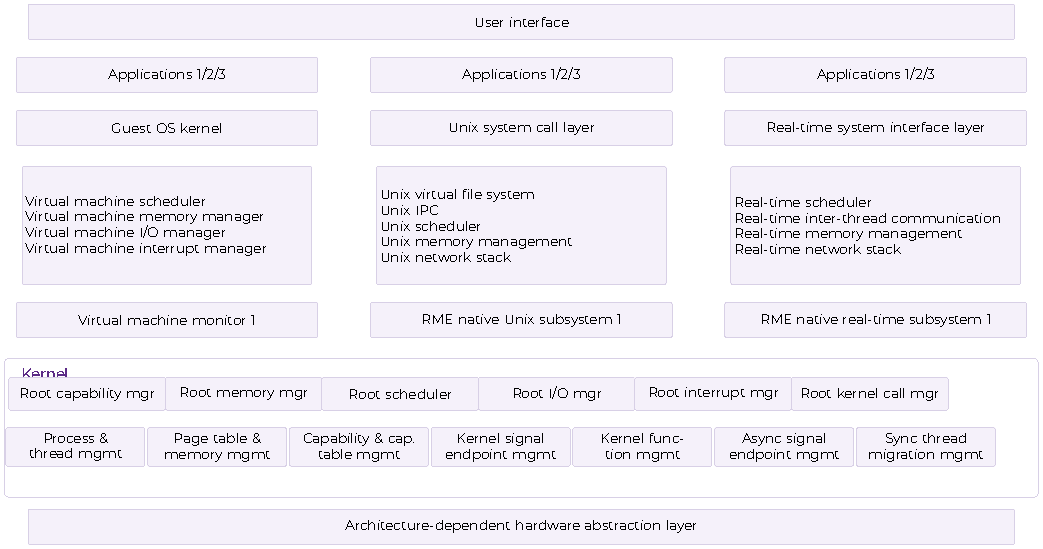
\includegraphics[width=0.90\textwidth]{Figure/image4.pdf}
    \caption{Brief architecture overview of RME}
    \label{fig:1-3-rme-architecture-overview}
\end{figure}

\section{Bibliography of This Chapter}\label{sec:1-bibliography}

\protect\phantomsection\label{cite:1-1}
{[}1{]}
T. N. B. Anh and S.-L. Tan, "Real-time operating systems for small
microcontrollers," IEEE micro, vol. 29, 2009.

\protect\phantomsection\label{cite:1-2}
{[}2{]} R. P. Kar, "Implementing the Rhealstone real-time benchmark,"
Dr. Dobb's Journal, vol. 15, pp. 46-55, 1990.

\protect\phantomsection\label{cite:1-3}
{[}3{]} T. J. Boger, Rhealstone benchmarking of FreeRTOS and the Xilinx
Zynq extensible processing platform: Temple University, 2013.

\protect\phantomsection\label{cite:1-4}
{[}4{]} G. Klein, K. Elphinstone, G. Heiser, J. Andronick, D. Cock, P.
Derrin, et al., "seL4: formal verification of an OS kernel," presented
at the Proceedings of the ACM SIGOPS 22nd symposium on Operating systems
principles, Big Sky, Montana, USA, 2009.

\protect\phantomsection\label{cite:1-5}
{[}5{]} U. Steinberg and B. Kauer, "NOVA: a microhypervisor-based secure
virtualization architecture," in Proceedings of the 5th European
conference on Computer systems, 2010, pp. 209-222.
